\chapter{Building Blocks of Logic} % Main chapter title

\label{Chapter1}

%-----------------------------------
%	section Classic Electrical Circuits
%-----------------------------------

\section{Classic Electrical Circuits}

\subsection{Signal Transmission}
Signal transmission in electronic circuits has a few major differences to that in the redstone circuits of Minecraft. First, most signals in the electric connections are bidirectional, while Minecraft, due to needing to use repeaters every few blocks, can only send signals in one direction. Secondly, Minecraft has no concept of closing a loop or shorting a circuit or anything related to voltage or amperage. Third, and most significantly, the speed difference of transmissions in the two subject matters are hard to imagine. The electromagnetic wave ripples through the wire at around 90 percent the speed of light, depending on the physical characteristics of the wire, which is ca. 2.7 * 10$^8$ m/s. The equivalent signal in Minecraft will travel at most at 18 blocks per RT, unless some unintended game mechanics are used, or 90 blocks per second in optimal conditions. A real CPU is around 4cm x 4cm in Area, while the CPU in this project takes up around 100 x 100 blocks, give or take. A signal can thus go from one side of the CPU to the opposite in 0.14 nanoseconds, or 1.4 * 10$^{-10}$s in a real CPU, whereas the Minecraft equivalent takes about 1.1s. Not even considering the increased complexity of the actual CPU, where a simpler one could be made significantly smaller, this equates to a speed ratio of 1 to 6.75 billion, or 9 orders of magnitude.

\subsection{Clock and Instruction Cycles}

In the x86 Instruction Set, a single instruction execution can cost from one up to dozens - and in rare cases, over a hundred - clock cycles. Take, for example, the Intel Pentium P5 processor \cite[Page 162 - Intel Pentium]{InstrTable_Agner}, a 32-bit processor running its clock at speeds from 60MHz up to 300 MHz. Its simplest operations, such as moving data from memory to register (MOV), can be executed in a single clock cycle, or simple logic operations, like adding a number from memory to a number from a register (ADD), takes only two clock cycles. Most operations, however, will take multiple clock cycles, though usually less than ten. An integer division (IDIV), however, the most expensive non-floating-point operation on the Pentium P5, will cost 46 clock cycles for two 32-bit longs. Some floating point operations are even more expensive, such as the floating point arctangent of a value (FPATAN) at a cost of 120-146 clock cycles. The reason for these high amounts of clock cycles is that some specific hardware components, like an integer division component, work in internal loops or on long conveyor belt type operations, and the instruction needs to wait until the entire operation is completed before it can access the computed result.

In some cases, mainly the conveyor belt type operations, the instructions can be pipelined, as they are often in actual conveyor belts, and the results can be spit out at a much higher frequency, but the delay between input and the corresponding output stays the same. In that case, the operation can be thought of as a classic Ford car manufacturing factory, where a car gets finished every few minutes or hours, but still may take days or weeks to make it through the entire system.

The reason for why even most of the simple instructions take multiple clock cycles is because of the complexity of the processor not allowing for direct connections between most components. The only method of communication between the major components that perform the logic is via the central data bus, and that can or should only be written to by one component at once. Thus, the instructions are split up into multiple cycles, so each piece of information can get through the processor to its destination.

The way the components are connected together in this CPU is not as simple as a single data bus, but where each component receives its input from all its sources directly and, by carefully setting the control bits, managing to never have any two sources arrive at the same destination and overwriting each other. While this does make the implementation of some instructions significantly harder and increasing the complexity in that regard, the benefits are much faster execution of instructions. This does limit the usage of slower hardware integrated circuits such as a multiplication or division, which thus need to be done in software. Adding any such hardware would drastically increase the complexity of the CPU and its instruction cycle. It is certainly in the scope of a Minecraft CPU, but not in the scope of this project. Thus, the slightly complex but easier to handle version of one clock cycle per instruction is the direction chosen for this CPU.

%-----------------------------------
%	section Minecraft Circuits
%-----------------------------------

\section{Minecraft Circuits} \label{ssec::MinecraftCircuits}

\subsection{Redstone Fundamentals}
Redstone, in its most basic form, is a wire that can be either on or off. If it is on, it holds a certain signal strength, between 0 and 15, which decreases by one each block. Through the redstone wire, it travels instantly, but once the signal strength reaches 0, it stops. Therefore, the signal needs to be renewed, at the cost of adding some delay. Whereas the game physics run on 20 ticks per second, i.e. the state of each block gets updated 20 times a second, the delays from redstone components take 2 ticks, or 1 redstone tick (RT), or a multiple of that. It is therefore common to refer to timings in redstone in RT. The fixed limit of 20 ticks per second can be modified using third-party mods, which can set the limit up to 500 ticks per second, though at that point the game usually cannot update itself fast enough to reach that limit.

\begin{figure}[!ht]
    \begin{center}
        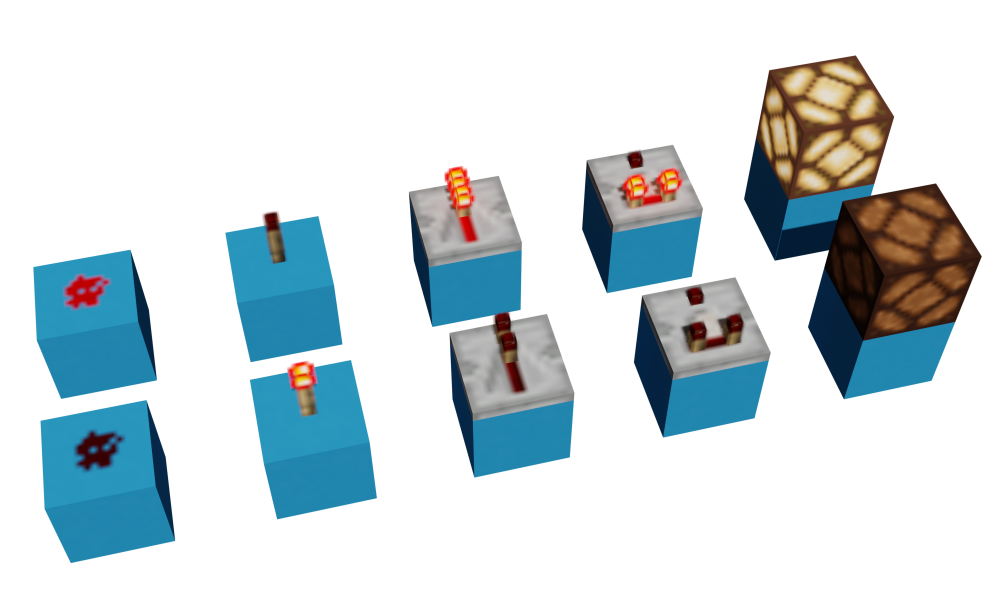
\includegraphics[width=0.7\textwidth]{Figures/Components-small.png}
        \caption[Five basic components]{From left to right: Redstone Dust, Redstone Torch, Repeater, Comparator and Redstone Lamp}
        \label{fig::RedstoneComponents}
    \end{center}
\end{figure}

\subsection{The Components} \label{ssec::Components}
There are five main components to redstone circuits: Redstone dust, the redstone torch, the repeater, the comparator and the redstone lamp as shown in Figure \ref{fig::RedstoneComponents}. The redstone torch will, in its normal state, emit a signal at full power to surrounding blocks, while powering the block above it in a way that the signal goes through the block and powers the surrounding blocks. If the block the redstone torch is connected to is powered, the redstone torch turns off, a property that is most commonly used as an inverter or a NOT gate.

The repeater, when powered from behind, emits a signal at full power into the block it is facing into, much like the redstone torch powers the block above it. The repeater can also be locked when powered from its side by another repeater. In the locked state, the repeater holds the power state it was in when it got locked and ignores any changes to its input, effectively storing one bit of data. The repeater can be manually configured to a specified delay between input and output within a range of 1-4RT, giving the user fine control over the time a transmission takes, something that is nearly impossible (and usually not wanted) in electronic circuits.

The comparator is possibly the most misunderstood redstone component by the playerbase, referring to its two modes and their interaction with signal strengths. The normal use case is to read out the signal strength from its input or the fill-level of the container behind it, where the fill-level is represented by a signal strength, and emit that signal strength in the front. Comparators can also receive inputs from the side, which interact differently depending on which mode the comparator is set to. In comparison mode, the comparator works as follows: If the signal from the main input is stronger than the signal from the side, it will output its received signal as it gets it, otherwise it doesn't emit a signal. In subtract mode, the comparator always subtracts the side input from the main output. This functionality allows it to be used a simple binary switch to control the flow of a signal. A common use case for the comparator in this CPU is as a pulse-width limiter, as shown in Figure \ref{fig::ExampleCircuits} on the right. When the circuit receives a signal, it first goes unhindered through the comparator with the standard 1RT delay, while the signal also passes through the repeater on the side, set to some delay. After the delay specified by the repeater, the signal is input on the side of the comparator at full strength, blocking any further transmission. This way, the maximum length of a signal going through the circuit is that specified by the repeater.

\subsection{Example Circuits} \label{ssec::ExampleCircuits}
Figure \ref{fig::ExampleCircuits} shows three important circuits. The first circuit is the classic AND gate nearly any redstone user in Minecraft will be familiar with. The two inputs control the redstone torches on the blocks, which act like inverters or NOT gates, i.e. an ON signal turns them off. As long as at least one torch emits a signal, the torch in the middle lane remains off and the output is off. Only when both inputs are on will the redstone dust in the middle unpower and allow the center torch to turn on again. The second circuit is the most commonly used XOR gate due to its simplicity, though it is pretty big. The comparators are set to subtract mode, so it will always output the main input minus the input from the side. This gate makes use of the fact that a signal loses strength over distance to check whether only one input is on. If only one input is on, the XOR gate outputs a signal. The best way to understand this gate is to simulate its function by manually counting the signal strengths at each comparator input. The last one is the aforementioned pulse limiter, as described in Section \ref{ssec::Components}, set to a pulse width of 3RT.

\begin{figure}[h]
    \begin{center}
        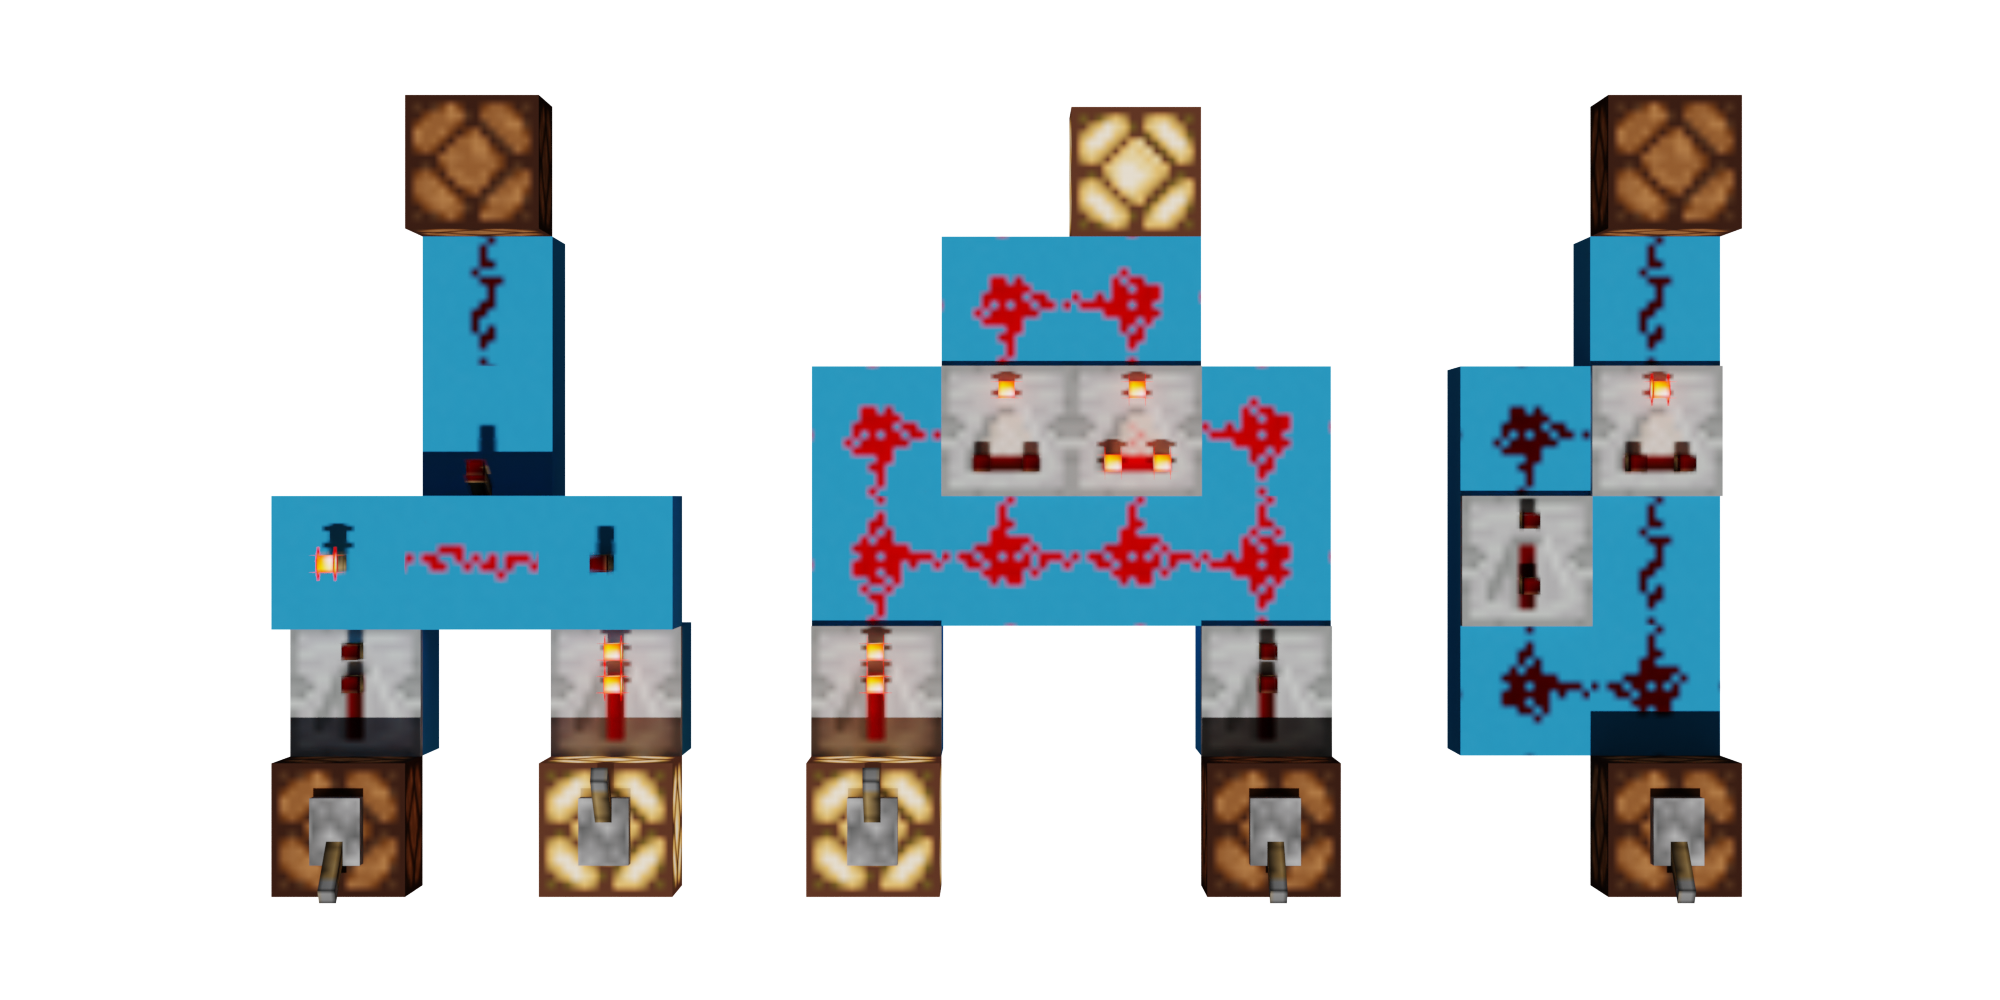
\includegraphics[width=0.9\textwidth]{Figures/ExampleCircuits.png}
        \caption{AND-Gate, XOR-Gate, Pulse-Width Limiter}
        \label{fig::ExampleCircuits}
    \end{center}
\end{figure}

